% =====================================================================
% University Project Presentation (LaTeX Beamer)
% Enhanced Design with Professional Styling
% Duration target: 10--15 minutes
% Compiler: pdflatex (recommended) or xelatex
% =====================================================================
\documentclass[aspectratio=169,11pt]{beamer}

\usetheme{Madrid}
\usecolortheme{seahorse}

\usepackage[T1]{fontenc}
\usepackage[utf8]{inputenc}
\usepackage{lmodern}
\usepackage{graphicx}
\usepackage{hyperref}
\usepackage{amsmath}
\usepackage{amssymb}
\usepackage{tikz}
\usetikzlibrary{calc}
\usepackage{xcolor}
\usepackage{booktabs}
\usepackage{pifont}

% --- Enhanced color scheme ---
\definecolor{accent1}{RGB}{25, 103, 210}
\definecolor{accent2}{RGB}{102, 51, 153}
\definecolor{accent3}{RGB}{0, 150, 136}
\definecolor{lightbg}{RGB}{240, 248, 255}
\definecolor{darktext}{RGB}{33, 33, 33}

% --- Custom theme colors ---
\setbeamercolor{frametitle}{bg=accent1, fg=white}
\setbeamercolor{title}{bg=accent1, fg=white}
\setbeamercolor{structure}{fg=accent1}
\setbeamercolor{itemize item}{fg=accent1}
\setbeamercolor{itemize subitem}{fg=accent3}
\setbeamercolor{block title}{bg=accent1, fg=white}
\setbeamercolor{block body}{bg=lightbg, fg=darktext}

% --- Custom fonts and spacing ---
\usefonttheme[onlymath]{serif}
\setbeamerfont{frametitle}{size=\Large, series=\bfseries}
\setbeamerfont{title}{size=\huge, series=\bfseries}
\setbeamerfont{author}{size=\large}

% --- Remove navigation symbols ---
\setbeamertemplate{navigation symbols}{}

% --- Footer with slide numbers ---
\setbeamertemplate{footline}{
  \hbox{%
    \begin{beamercolorbox}[wd=\paperwidth,ht=2.5ex,dp=1ex]{footline}%
      \hspace*{2em}%
      {\footnotesize Quincaillerie App}%
      \hfill%
      {\footnotesize \insertframenumber{} / \inserttotalframenumber}%
      \hspace*{2em}%
    \end{beamercolorbox}%
  }%
}

% --- Checkmark command ---
\newcommand{\cmark}{\textcolor{accent3}{\ding{51}}}

\title[Quincaillerie App]{Quincaillerie Management Web Application\\Inventory \& Billing System}
\author{Farouk BENKHELIFA}
\institute{ENSTTIC}
\date{Academic Year 2025/2026}

\begin{document}

% =====================================================================
% SLIDE 1: Title slide
% =====================================================================
\begin{frame}[plain]
\begin{tikzpicture}[remember picture, overlay]
  \fill[accent1] (current page.south west) rectangle (current page.north east);
  \fill[white] (current page.south west) rectangle ($ (current page.south east) + (0, 0.8cm) $);
  \fill[accent3, opacity=0.15] ($ (current page.north west) + (2cm, -2cm) $) circle (4cm);
  \fill[accent2, opacity=0.1] ($ (current page.south east) + (-3cm, 3cm) $) circle (3cm);
\end{tikzpicture}

\vspace{1.5cm}
\begin{center}
  {\huge \bfseries \textcolor{white}{Quincaillerie Management}}\\[0.3cm]
  {\huge \bfseries \textcolor{white}{Web Application}}\\[0.6cm]
  {\Large \textcolor{lightbg}{Inventory \& Billing System}}\\[2cm]
  {\large \textcolor{white}{\textbf{Farouk BENKHELIFA}}}\\[0.2cm]
  {\normalsize \textcolor{lightbg}{ENSTTIC}}\\[1.5cm]
  {\small \textcolor{lightbg}{Academic Year 2025/2026}}
\end{center}
\end{frame}

% =====================================================================
% SLIDE 2: Context & Problem
% =====================================================================
\begin{frame}{Context \& Problem}

\begin{columns}[T]
  \begin{column}{0.48\textwidth}
    \textbf{\textcolor{accent1}{The Challenge}}
    \begin{itemize}
      \item Hardware stores manage \alert{diverse inventory}
      \item Manual tracking leads to errors
      \item Slow and inefficient operations
    \end{itemize}
  \end{column}
  
  \begin{column}{0.48\textwidth}
    \textbf{\textcolor{accent1}{Key Pain Points}}
    \begin{itemize}
      \item \textcolor{accent2}{Inaccurate} stock levels
      \item \alert{Late} reordering decisions
      \item Missing \textcolor{accent3}{audit trail}
      \item Slow product search
      \item Inconsistent invoices
    \end{itemize}
  \end{column}
\end{columns}

\vspace{0.8cm}

\begin{block}{Business Impact}
  Without proper system: \textbf{lost sales}, \textbf{overstocking}, and \textbf{accounting errors}
\end{block}

\end{frame}

% =====================================================================
% SLIDE 3: Project Objectives
% =====================================================================
\begin{frame}{Project Objectives}

\begin{enumerate}
  \item[\textcolor{accent1}{\textbf{1.}}] \textbf{Core Functionality}
  \begin{itemize}
    \item Product catalog management
    \item Invoice creation and printing
    \item Automatic stock updates with traceability
  \end{itemize}
  
  \vspace{0.3cm}
  
  \item[\textcolor{accent1}{\textbf{2.}}] \textbf{User Experience}
  \begin{itemize}
    \item Optimized for \alert{non-technical users}
    \item Fast and responsive interface
  \end{itemize}
  
  \vspace{0.3cm}
  
  \item[\textcolor{accent1}{\textbf{3.}}] \textbf{Advanced Features}
  \begin{itemize}
    \item Multilingual support (French / Arabic)
    \item Light / Dark mode themes
    \item Strong data consistency (transactions)
  \end{itemize}
\end{enumerate}

\end{frame}

% =====================================================================
% SLIDE 4: Technologies Used
% =====================================================================
\begin{frame}{Technologies Used}

\begin{columns}[T]
  \begin{column}{0.32\textwidth}
    \begin{block}{Backend}
      \textbf{\textcolor{accent1}{Laravel}}
      \begin{itemize}
        \item[\cmark] MVC Architecture
        \item[\cmark] Routing \& Auth
        \item[\cmark] ORM (Eloquent)
        \item[\cmark] Migrations
      \end{itemize}
    \end{block}
  \end{column}
  
  \begin{column}{0.32\textwidth}
    \begin{block}{Frontend}
      \textbf{\textcolor{accent1}{React + MUI}}
      \begin{itemize}
        \item[\cmark] Component-based
        \item[\cmark] Material UI
        \item[\cmark] Responsive
        \item[\cmark] Accessible
      \end{itemize}
    \end{block}
  \end{column}
  
  \begin{column}{0.32\textwidth}
    \begin{block}{Infrastructure}
      \textbf{\textcolor{accent1}{Stack}}
      \begin{itemize}
        \item[\cmark] MySQL Database
        \item[\cmark] Inertia.js
        \item[\cmark] Vite (Build)
        \item[\cmark] Laragon (Dev)
      \end{itemize}
    \end{block}
  \end{column}
\end{columns}

\end{frame}

% =====================================================================
% SLIDE 5: System Architecture
% =====================================================================
\begin{frame}{System Architecture}

\begin{columns}[T]
  \begin{column}{0.45\textwidth}
    \vspace{0.5cm}
    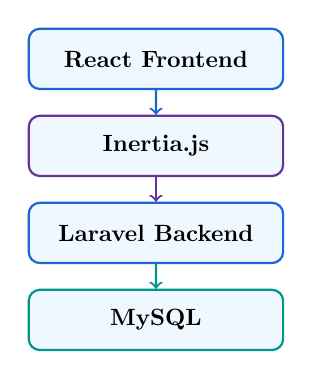
\begin{tikzpicture}[scale=0.85, transform shape]
      \node[draw=accent1, fill=lightbg, thick, rounded corners, minimum width=3.8cm, minimum height=0.9cm] (client) at (0, 4) {\textbf{React Frontend}};
      \node[draw=accent2, fill=lightbg, thick, rounded corners, minimum width=3.8cm, minimum height=0.9cm] (inertia) at (0, 2.7) {\textbf{Inertia.js}};
      \node[draw=accent1, fill=lightbg, thick, rounded corners, minimum width=3.8cm, minimum height=0.9cm] (laravel) at (0, 1.4) {\textbf{Laravel Backend}};
      \node[draw=accent3, fill=lightbg, thick, rounded corners, minimum width=3.8cm, minimum height=0.9cm] (database) at (0, 0.1) {\textbf{MySQL}};
      
      \draw[->, thick, accent1] (client) -- (inertia);
      \draw[->, thick, accent2] (inertia) -- (laravel);
      \draw[->, thick, accent3] (laravel) -- (database);
    \end{tikzpicture}
  \end{column}
  
  \begin{column}{0.52\textwidth}
    \textbf{\textcolor{accent1}{How It Works}}
    \begin{itemize}
      \item \textbf{Laravel:} routes, auth, transactions
      \item \textbf{Inertia:} server routing + SPA feel
      \item \textbf{React:} dynamic UI rendering
      \item \textbf{MySQL:} normalized data storage
    \end{itemize}
    
    \vspace{0.5cm}
    
    \begin{block}{Key Benefit}
      No separate API needed --- single codebase with SPA experience
    \end{block}
  \end{column}
\end{columns}

\end{frame}

% =====================================================================
% SLIDE 6: Database Design
% =====================================================================
\begin{frame}{Database Design}

\begin{columns}[T]
  \begin{column}{0.48\textwidth}
    \textbf{\textcolor{accent1}{Core Entities}}
    \begin{itemize}
      \item Product
      \item Category
      \item Supplier
      \item Worker
    \end{itemize}
    
    \vspace{0.4cm}
    
    \textbf{\textcolor{accent1}{Billing}}
    \begin{itemize}
      \item Bill (header)
      \item BillItem (lines)
    \end{itemize}
  \end{column}
  
  \begin{column}{0.48\textwidth}
    \textbf{\textcolor{accent1}{Audit \& Config}}
    \begin{itemize}
      \item InventoryMovement
      \begin{itemize}
        \item sale, adjustment, return
      \end{itemize}
    \end{itemize}
    
    \vspace{0.4cm}
    
    \textbf{\textcolor{accent1}{Settings}}
    \begin{itemize}
      \item Store identity
      \item Invoice footer
    \end{itemize}
  \end{column}
\end{columns}

\end{frame}

% =====================================================================
% SLIDE 7: Main Features - Dashboard & Products
% =====================================================================
\begin{frame}{Main Features --- Dashboard \& Products}

\begin{itemize}
  \item \textbf{Dashboard:} statistics, low stock alerts, recent activity
  \item \textbf{Products:} CRUD, search, categories, suppliers, images
  \item \textbf{Inventory:} stock adjustments with traceability
\end{itemize}

\vspace{0.5cm}

\begin{columns}
  \begin{column}{0.48\textwidth}
    \begin{center}
    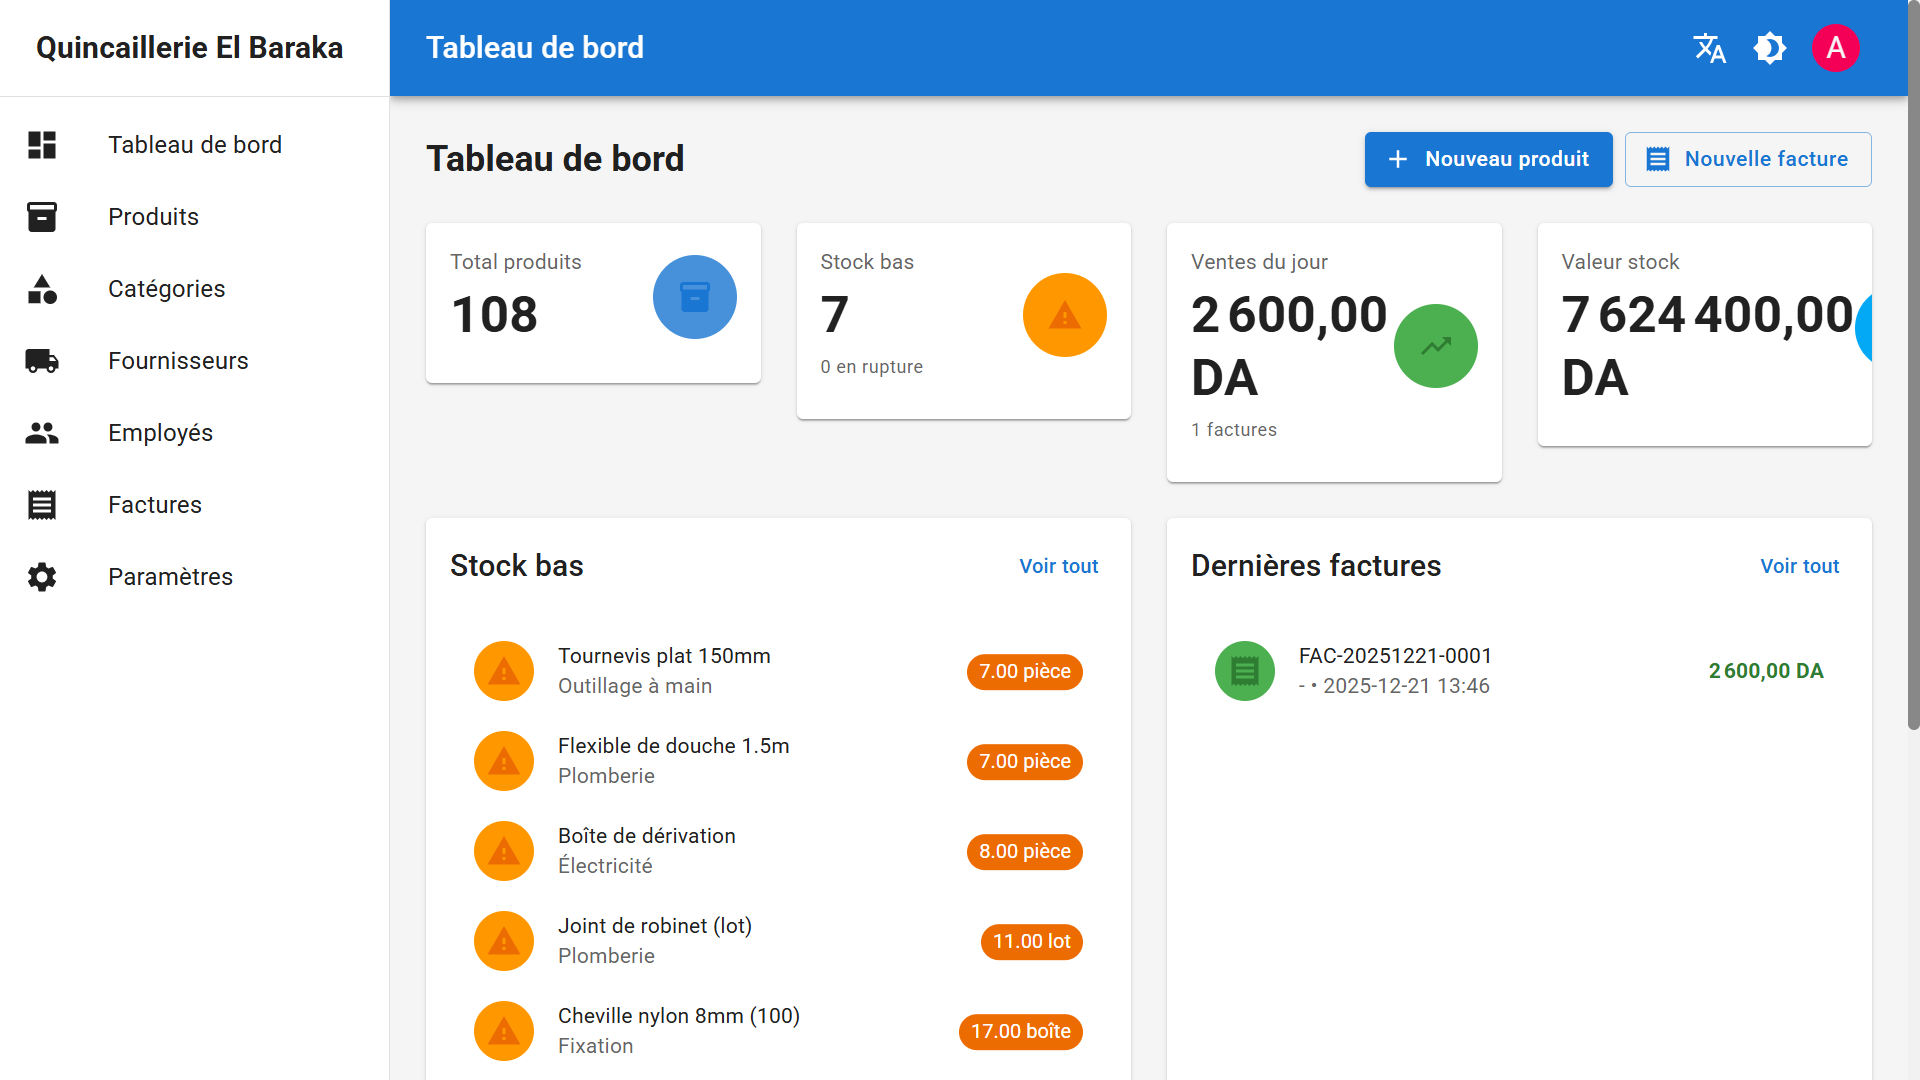
\includegraphics[width=\textwidth]{figures/dashboard.png}
    \end{center}
  \end{column}
  
  \begin{column}{0.48\textwidth}
    \begin{center}
    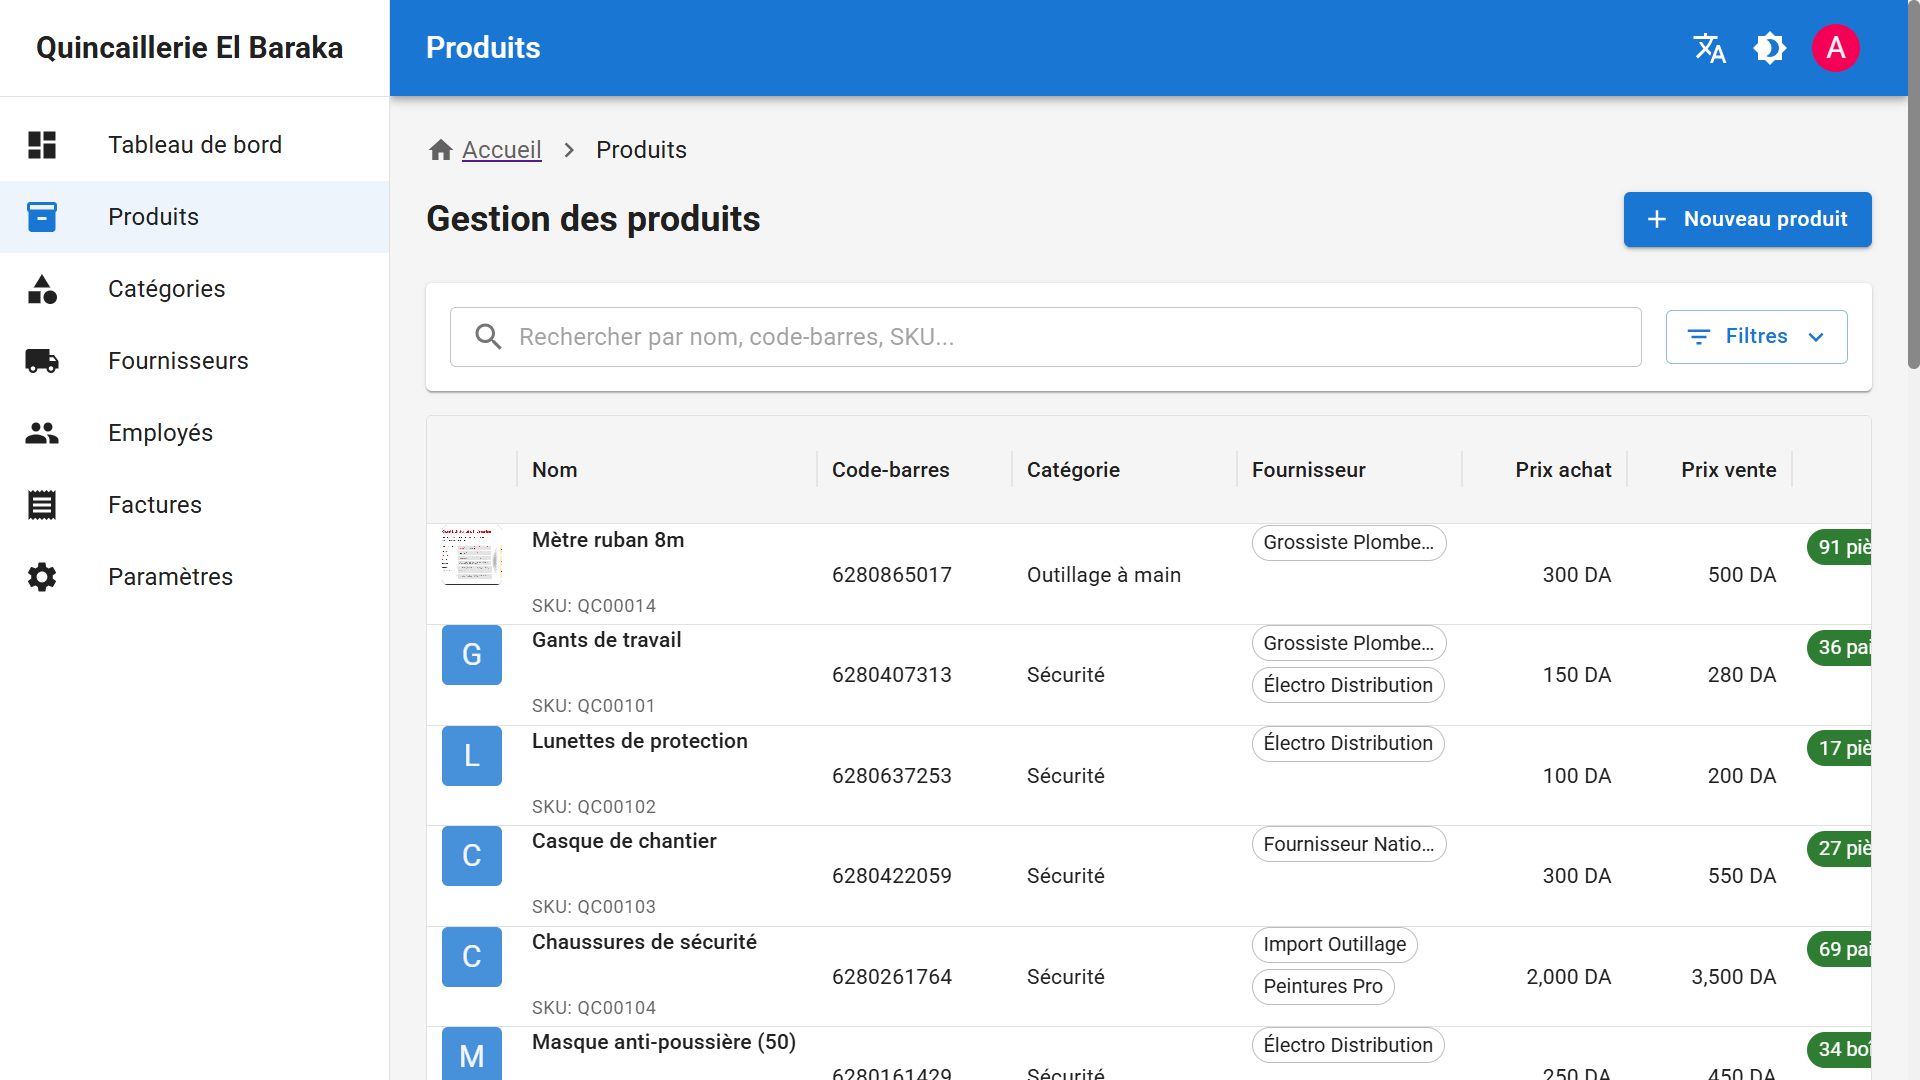
\includegraphics[width=\textwidth]{figures/products-list.png}
    \end{center}
  \end{column}
\end{columns}

\end{frame}

% =====================================================================
% SLIDE 8: Main Features - Billing
% =====================================================================
\begin{frame}{Main Features --- Billing}

\begin{itemize}
  \item \textbf{Bill creation:} multi-product selection, quantity input
  \item \textbf{Totals:} subtotal, discount, tax, grand total
  \item \textbf{Actions:} print preview, PDF export (FR/AR), edit, cancel
\end{itemize}

\vspace{0.5cm}

\begin{columns}
  \begin{column}{0.48\textwidth}
    \begin{center}
    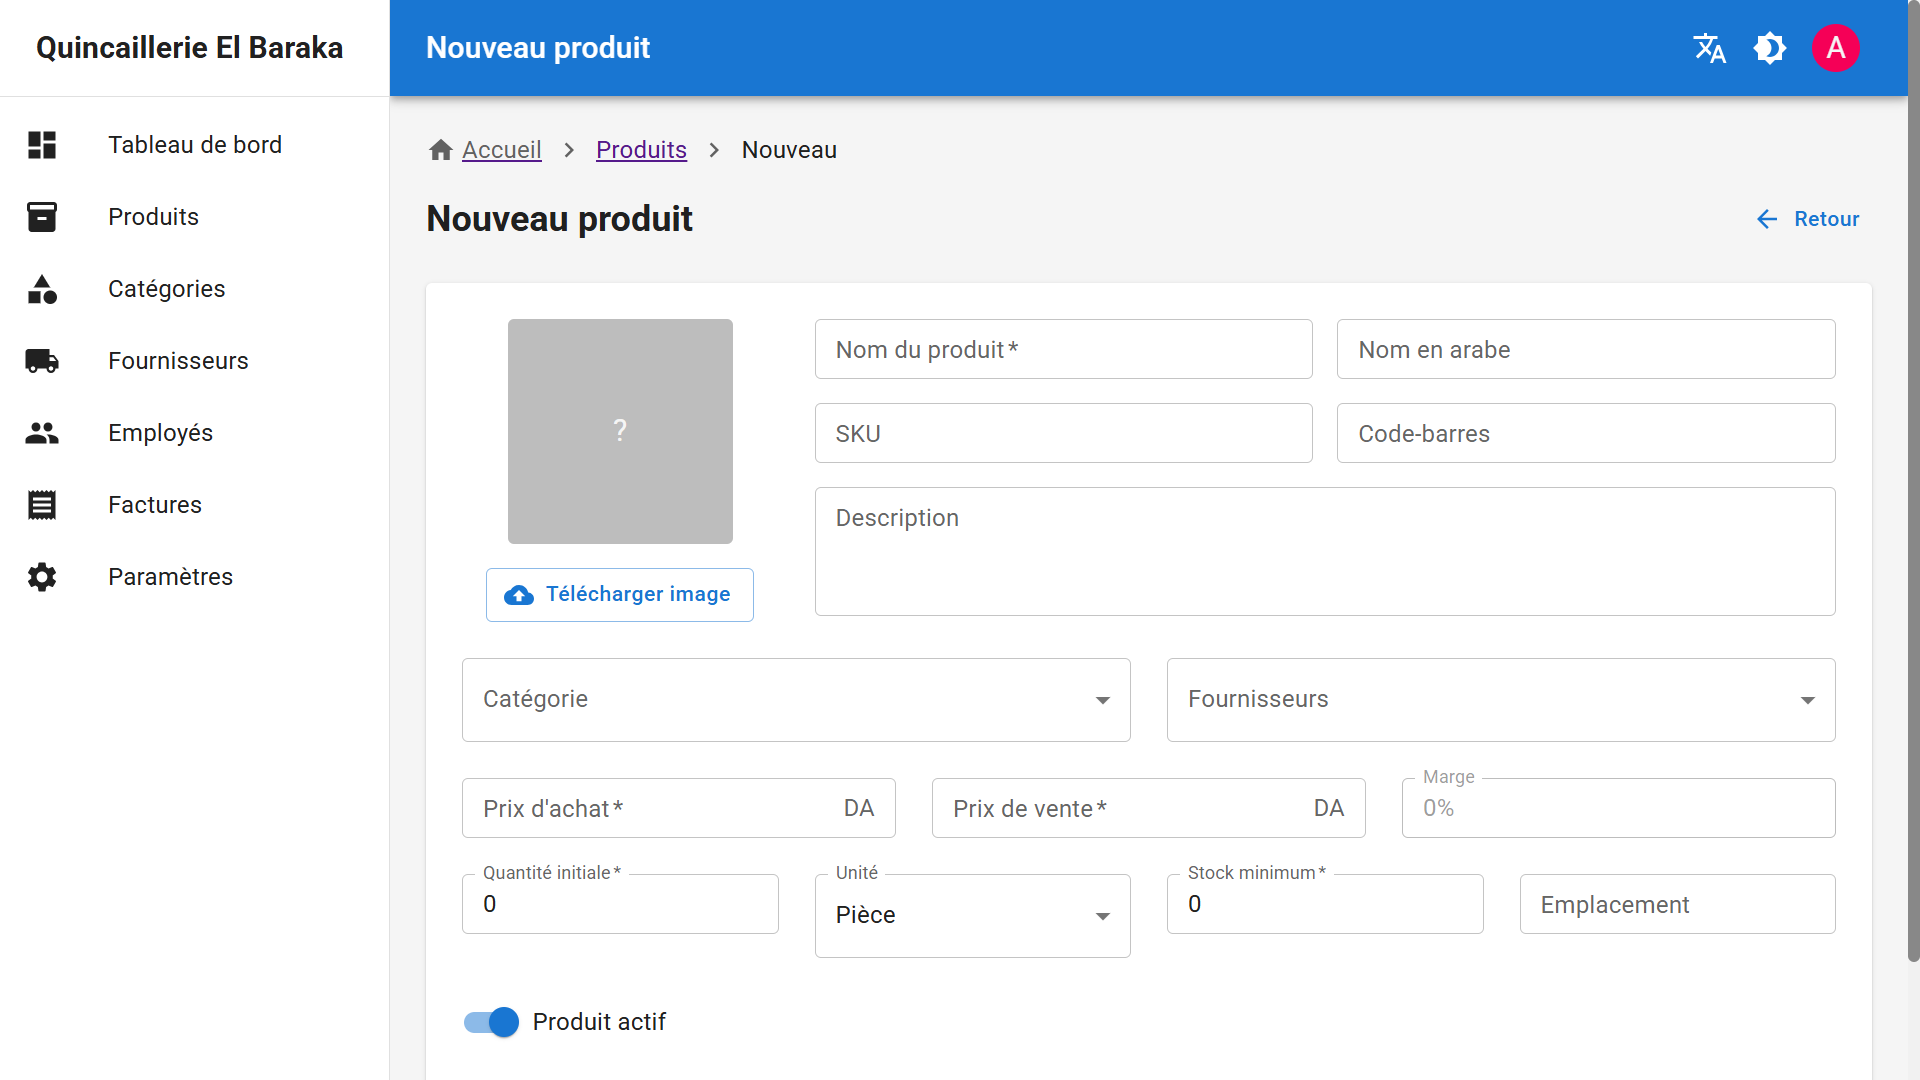
\includegraphics[width=\textwidth]{figures/product-create.png}
    \end{center}
  \end{column}
  
  \begin{column}{0.48\textwidth}
    \begin{center}
    \includegraphics[width=\textwidth]{figures/bill-print.png}
    \end{center}
  \end{column}
\end{columns}

\end{frame}

% =====================================================================
% SLIDE 9: Multilingual & Theme Features
% =====================================================================
\begin{frame}{Multilingual \& Theme Features}

\begin{columns}[T]
  \begin{column}{0.48\textwidth}
    \textbf{\textcolor{accent1}{Language Support}}
    \begin{itemize}
      \item[\cmark] French UI
      \item[\cmark] Arabic translations
      \item[\cmark] Context-aware labels
    \end{itemize}
    
    \vspace{0.3cm}
    
    \textbf{Design Choice:}\\
    {\small Layout stays \textbf{LTR}; only text changes}
  \end{column}
  
  \begin{column}{0.48\textwidth}
    \textbf{\textcolor{accent1}{Theme Modes}}
    \begin{itemize}
      \item[\cmark] Light mode (default)
      \item[\cmark] Dark mode
      \item[\cmark] Toggle in sidebar
    \end{itemize}
    
    \vspace{0.3cm}
    
    \textbf{Benefit:}\\
    {\small Better readability in all conditions}
  \end{column}
\end{columns}

\end{frame}

% =====================================================================
% SLIDE 10: Demo Plan
% =====================================================================
\begin{frame}{Demo Plan (Live)}

\begin{enumerate}
  \item \textbf{Login} with test user credentials
  
  \vspace{0.2cm}
  
  \item \textbf{Dashboard:} view statistics, low stock alerts
  
  \vspace{0.2cm}
  
  \item \textbf{Products:} search, view details, check image display
  
  \vspace{0.2cm}
  
  \item \textbf{Create Bill:} add multiple items, adjust quantities, validate
  
  \vspace{0.2cm}
  
  \item \textbf{Bill Details:} print preview, PDF export
  
  \vspace{0.2cm}
  
  \item \textbf{Settings:} update store info, verify on invoice
\end{enumerate}

\end{frame}

% =====================================================================
% SLIDE 11: Conclusion & Future Work
% =====================================================================
\begin{frame}{Conclusion \& Future Work}

\begin{block}{Conclusion}
  \begin{itemize}
    \item \textcolor{accent1}{\textbf{Complete}} local inventory and billing system
    \item \textbf{Data consistency} ensured through transactions
    \item \textbf{Bilingual} UI and print-ready invoices
  \end{itemize}
\end{block}

\vspace{0.4cm}

\begin{block}{Future Improvements}
  \begin{columns}[T]
    \begin{column}{0.48\textwidth}
      \begin{itemize}
        \item Role-based permissions
        \item Advanced analytics
        \item Backup/export workflows
      \end{itemize}
    \end{column}
    
    \begin{column}{0.48\textwidth}
      \begin{itemize}
        \item Barcode scanner support
        \item Offline packaging
        \item Mobile responsive UI
      \end{itemize}
    \end{column}
  \end{columns}
\end{block}

\end{frame}

% =====================================================================
% SLIDE 12: Thank You
% =====================================================================
\begin{frame}[plain]
\begin{tikzpicture}[remember picture, overlay]
  \fill[accent1] (current page.south west) rectangle (current page.north east);
  \fill[accent2, opacity=0.2] ($ (current page.north west) + (2cm, -2cm) $) circle (3cm);
  \fill[accent3, opacity=0.15] ($ (current page.south east) + (-2cm, 2cm) $) circle (2.5cm);
\end{tikzpicture}

\vspace{2.5cm}
\begin{center}
  {\Huge \bfseries \textcolor{white}{Thank You}}\\[1cm]
  {\Large \textcolor{lightbg}{Questions?}}\\[2cm]
  {\normalsize \textcolor{lightbg}{Farouk BENKHELIFA}}\\[0.2cm]
  {\small \textcolor{lightbg}{ENSTTIC --- 2025/2026}}
\end{center}
\end{frame}

\end{document}
